\documentclass[tikz]{standalone}

\usepackage[T1]{fontenc}
\usepackage[english]{babel}

\usepackage{tikz}

\begin{document}

	\begin{tikzpicture}
		\node[visible on=<1>] (image) {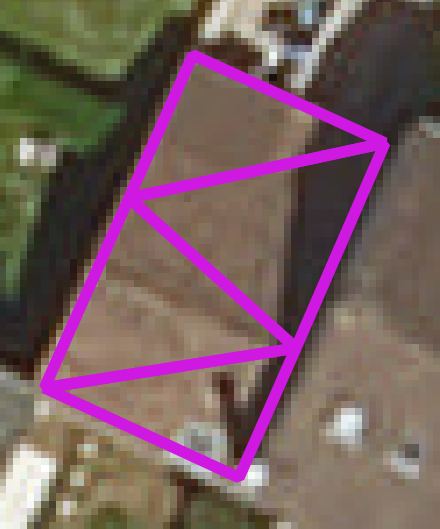
\includegraphics[width=5cm, angle=270]{images/introduction/graphical_abstract/orthoprojection}};
		\path (image.south) node[anchor=north, visible on=<1>, text width=5cm, align=center] (image_legend) {\scriptsize Nadir projection on orthoimage.};
		\path (image_legend) node[visible on=<3>, text width=5cm, align=center] (image_legend) {\scriptsize Histogram over Edges.};
		\path (image_legend) node[visible on=<4>, text width=5cm, align=center] (image_legend) {\scriptsize Histogram over Facets.};
		\path (image_legend) node[visible on=<5>, text width=5cm, align=center] (image_legend) {\scriptsize Global histogram.};

		\path (image) + (-.25, 0) node[visible on=<2>] (pixel_segment) {\includestandalone[width=4cm]{figures/features/image_based}};
		\path (pixel_segment.south) node[anchor=north, visible on=<2>, align=center] (image_legend) {
			\scriptsize
			\begin{tabular}{c c c c}
				\textcolor{green!30}{\(\blacksquare\)} & intersecting pixel. & \textcolor{red}{\(\blacksquare\)} & model edge.\\
				\textcolor{purple}{\(\nabla I\)} & local gradient. & \textcolor{black}{\(\vec{n}\)} & edge \acrshort{acr::2d} normal.
			\end{tabular}
		};

		\path (image) node[visible on=<3-5>] (segment_hist) {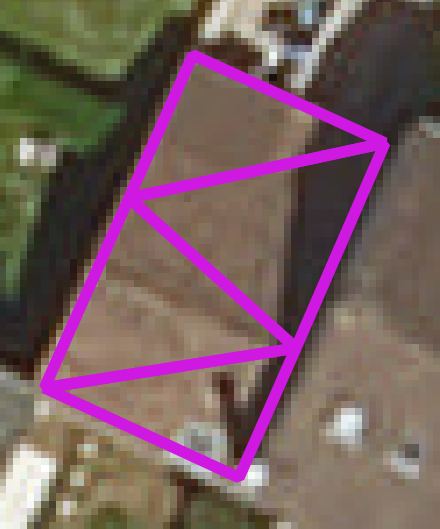
\includegraphics[width=5cm, angle=270]{images/introduction/graphical_abstract/orthoprojection}};

		\path (image) + (2.33, -1) node[visible on =<3>] (segment_hist_1) {
			\resizebox{.75cm}{.75cm}{
				\begin{tikzpicture}background rectangle/.style={fill=white}, show background rectangle
					\begin{axis}[
						area style,
						axis background/.style={fill=white},
						ymin=0,
						ytick=\empty,
						xtick=\empty,
						visible on=<3>
					]
						\addplot+[ycomb, blue, mark=*, mark options={scale=2, fill=blue}, very thick] plot coordinates {
							(-8, 3623)
							(-7, 546)
							(-6, 159)
							(-5, 182)
							(-4, 70)
						};
					\end{axis}
				\end{tikzpicture}
			}
		};
		\path (image) + (-2.16, 1.16) node[visible on =<3>] (segment_hist_2) {
			\resizebox{.75cm}{.75cm}{
				\begin{tikzpicture}background rectangle/.style={fill=white}, show background rectangle
					\begin{axis}[
						area style,
						axis background/.style={fill=white},
						ymin=0,
						ytick=\empty,
						xtick=\empty,
						visible on=<3>
					]
						\addplot+[ycomb, blue, mark=*, mark options={scale=2, fill=blue}, very thick] plot coordinates {
							(-8, 3623)
							(-7, 546)
							(-6, 1595)
							(-5, 182)
							(-4, 4151)
						};
					\end{axis}
				\end{tikzpicture}
			}
		};
		\path (image) + (-2.16, -.83) node[visible on =<3>] (segment_hist_3) {
			\resizebox{.75cm}{.75cm}{
				\begin{tikzpicture}background rectangle/.style={fill=white}, show background rectangle
					\begin{axis}[
						area style,
						axis background/.style={fill=white},
						ymin=0,
						ytick=\empty,
						xtick=\empty,
						visible on=<3>
					]
						\addplot+[ycomb, blue, mark=*, mark options={scale=2, fill=blue}, very thick] plot coordinates {
							(-8, 3623)
							(-7, 5446)
							(-6, 159)
							(-5, 1852)
							(-4, 70)
						};
					\end{axis}
				\end{tikzpicture}
			}
		};
		\path (image) + (.33, -1.66) node[visible on =<3>] (segment_hist_4) {
			\resizebox{.75cm}{.75cm}{
				\begin{tikzpicture}background rectangle/.style={fill=white}, show background rectangle
					\begin{axis}[
						area style,
						axis background/.style={fill=white},
						ymin=0,
						ytick=\empty,
						xtick=\empty,
						visible on=<3>
					]
						\addplot+[ycomb, blue, mark=*, mark options={scale=2, fill=blue}, very thick] plot coordinates {
							(-8, 3623)
							(-7, 546)
							(-6, 159)
							(-5, 182)
							(-4, 5670)
						};
					\end{axis}
				\end{tikzpicture}
			}
		};
		\path (image) + (-.33, 1.66) node[visible on =<3>] (segment_hist_5) {
			\resizebox{.75cm}{.75cm}{
				\begin{tikzpicture}background rectangle/.style={fill=white}, show background rectangle
					\begin{axis}[
						area style,
						axis background/.style={fill=white},
						ymin=0,
						ytick=\empty,
						xtick=\empty,
						visible on=<3>
					]
						\addplot+[ycomb, blue, mark=*, mark options={scale=2, fill=blue}, very thick] plot coordinates {
							(-8, 3623)
							(-7, 546)
							(-6, 159)
							(-5, 3182)
							(-4, 70)
						};
					\end{axis}
				\end{tikzpicture}
			}
		};
		\path (image) + (1.66, 1) node[visible on =<3>] (segment_hist_6) {
			\resizebox{.75cm}{.75cm}{
				\begin{tikzpicture}background rectangle/.style={fill=white}, show background rectangle
					\begin{axis}[
						area style,
						axis background/.style={fill=white},
						ymin=0,
						ytick=\empty,
						xtick=\empty,
						visible on=<3>
					]
						\addplot+[ycomb, blue, mark=*, mark options={scale=2, fill=blue}, very thick] plot coordinates {
							(-8, 323)
							(-7, 5426)
							(-6, 159)
							(-5, 1582)
							(-4, 70)
						};
					\end{axis}
				\end{tikzpicture}
			}
		};
		\path (image) + (1.16, -.33) node[visible on =<3>] (segment_hist_7) {
			\resizebox{.75cm}{.75cm}{
				\begin{tikzpicture}background rectangle/.style={fill=white}, show background rectangle
					\begin{axis}[
						area style,
						axis background/.style={fill=white},
						ymin=0,
						ytick=\empty,
						xtick=\empty,
						visible on=<3>
					]
						\addplot+[ycomb, blue, mark=*, mark options={scale=2, fill=blue}, very thick] plot coordinates {
							(-8, 23)
							(-7, 5456)
							(-6, 159)
							(-5, 182)
							(-4, 70)
						};
					\end{axis}
				\end{tikzpicture}
			}
		};
		\path (image) node[visible on =<3>] (segment_hist_8) {
			\resizebox{.75cm}{.75cm}{
				\begin{tikzpicture}background rectangle/.style={fill=white}, show background rectangle
					\begin{axis}[
						area style,
						axis background/.style={fill=white},
						ymin=0,
						ytick=\empty,
						xtick=\empty,
						visible on=<3>
					]
						\addplot+[ycomb, blue, mark=*, mark options={scale=2, fill=blue}, very thick] plot coordinates {
							(-8, 33)
							(-7, 546)
							(-6, 1059)
							(-5, 1482)
							(-4, 70)
						};
					\end{axis}
				\end{tikzpicture}
			}
		};
		\path (image) + (-1, .66) node[visible on =<3>] (segment_hist_9) {
			\resizebox{.75cm}{.75cm}{
				\begin{tikzpicture}background rectangle/.style={fill=white}, show background rectangle
					\begin{axis}[
						area style,
						axis background/.style={fill=white},
						ymin=0,
						ytick=\empty,
						xtick=\empty,
						visible on=<3>
					]
						\addplot+[ycomb, blue, mark=*, mark options={scale=2, fill=blue}, very thick] plot coordinates {
							(-8, 3623)
							(-7, 546)
							(-6, 159)
							(-5, 182)
							(-4, 70)
						};
					\end{axis}
				\end{tikzpicture}
			}
		};

		\path (image) + (1.56, 0) node[visible on =<4>] (facet_hist_1) {
			\resizebox{.75cm}{.75cm}{
				\begin{tikzpicture}background rectangle/.style={fill=white}, show background rectangle
					\begin{axis}[
						area style,
						axis background/.style={fill=white},
						ymin=0,
						ytick=\empty,
						xtick=\empty,
						visible on=<4>
					]
						\addplot+[ycomb, blue, mark=*, mark options={scale=2, fill=teal}, teal, very thick] plot coordinates {
							(-8, 3623)
							(-7, 546)
							(-6, 159)
							(-5, 182)
							(-4, 70)
						};
					\end{axis}
				\end{tikzpicture}
			}
		};
		\path (image) + (.33, -.5) node[visible on =<4>] (facet_hist_2) {
			\resizebox{.75cm}{.75cm}{
				\begin{tikzpicture}background rectangle/.style={fill=white}, show background rectangle
					\begin{axis}[
						area style,
						axis background/.style={fill=white},
						ymin=0,
						ytick=\empty,
						xtick=\empty,
						visible on=<4>
					]
						\addplot+[ycomb, blue, mark=*, mark options={scale=2, fill=teal}, teal, very thick] plot coordinates {
							(-8, 373)
							(-7, 546)
							(-6, 12)
							(-5, 182)
							(-4, 2842)
						};
					\end{axis}
				\end{tikzpicture}
			}
		};
		\path (image) + (-.5, .83) node[visible on =<4>] (facet_hist_3) {
			\resizebox{.75cm}{.75cm}{
				\begin{tikzpicture}background rectangle/.style={fill=white}, show background rectangle
					\begin{axis}[
						area style,
						axis background/.style={fill=white},
						ymin=0,
						ytick=\empty,
						xtick=\empty,
						visible on=<4>
					]
						\addplot+[ycomb, blue, mark=*, mark options={scale=2, fill=teal}, teal, very thick] plot coordinates {
							(-8, 623)
							(-7, 546)
							(-6, 1595)
							(-5, 182)
							(-4, 4151)
						};
					\end{axis}
				\end{tikzpicture}
			}
		};
		\path (image) + (-1.6, 0.16) node[visible on =<4>] (facet_hist_4) {
			\resizebox{.75cm}{.75cm}{
				\begin{tikzpicture}background rectangle/.style={fill=white}, show background rectangle
					\begin{axis}[
						area style,
						axis background/.style={fill=white},
						ymin=0,
						ytick=\empty,
						xtick=\empty,
						visible on=<4>
					]
						\addplot+[ycomb, blue, mark=*, mark options={scale=2, fill=teal}, teal, very thick] plot coordinates {
							(-8, 33)
							(-7, 546)
							(-6, 1595)
							(-5, 182)
							(-4, 41)
						};
					\end{axis}
				\end{tikzpicture}
			}
		};
		\path (image) + (-1.6, 0.16) node[visible on =<4>] (facet_hist_4) {
			\resizebox{.75cm}{.75cm}{
				\begin{tikzpicture}background rectangle/.style={fill=white}, show background rectangle
					\begin{axis}[
						area style,
						axis background/.style={fill=white},
						ymin=0,
						ytick=\empty,
						xtick=\empty,
						visible on=<4>
					]
						\addplot+[ycomb, blue, mark=*, mark options={scale=2, fill=teal}, teal, very thick] plot coordinates {
							(-8, 33)
							(-7, 546)
							(-6, 1595)
							(-5, 182)
							(-4, 41)
						};
					\end{axis}
				\end{tikzpicture}
			}
		};
		
		\path (image) node[visible on =<5>] (whole_hist) {
			\resizebox{1.5cm}{1.5cm}{
				\begin{tikzpicture}background rectangle/.style={fill=white}, show background rectangle
					\begin{axis}[
						area style,
						axis background/.style={fill=white},
						ymin=0,
						ytick=\empty,
						xtick=\empty,
						visible on=<5>
					]
						\addplot+[ybar interval,mark=no] plot coordinates {
							(-15, 0) 
							(-14, 0)
							(-13, 876)
							(-12, 366)
							(-11, 593)
							(-10, 675)
							(-9, 2231)
							(-8, 33)
							(-7, 546)
							(-6, 195)
							(-5, 182)
							(-4, 3641)
							(-3, 54)
							(-2, 123)
							(-1, 3815)
							(0, 4291)
							(1, 211)
							(2, 10)
							(3, 0)
							(4, 0)
							(5, 0)
							(6, 0)
							(7, 0)
							(8, 0)
						};
					\end{axis}
				\end{tikzpicture}
			}
		};
		\path (image) node[visible on =<6>] (whole_hist) {
			\resizebox{4cm}{3cm}{
				\begin{tikzpicture}background rectangle/.style={fill=white}, show background rectangle
					\begin{axis}[
						area style,
						axis background/.style={fill=white},
						ymin=0,
						visible on=<6>
					]
						\addplot+[ybar interval,mark=no] plot coordinates {
							(-15, 0) 
							(-14, 0)
							(-13, 876)
							(-12, 366)
							(-11, 593)
							(-10, 675)
							(-9, 2231)
							(-8, 33)
							(-7, 546)
							(-6, 195)
							(-5, 182)
							(-4, 3641)
							(-3, 54)
							(-2, 123)
							(-1, 3815)
							(0, 4291)
							(1, 211)
							(2, 10)
							(3, 0)
							(4, 0)
							(5, 0)
							(6, 0)
							(7, 0)
							(8, 0)
						};
					\end{axis}
				\end{tikzpicture}
			}
		};
	\end{tikzpicture}
\end{document}
